\begin{figure}[th]
	\centering
	\resizebox{1\columnwidth}{!}{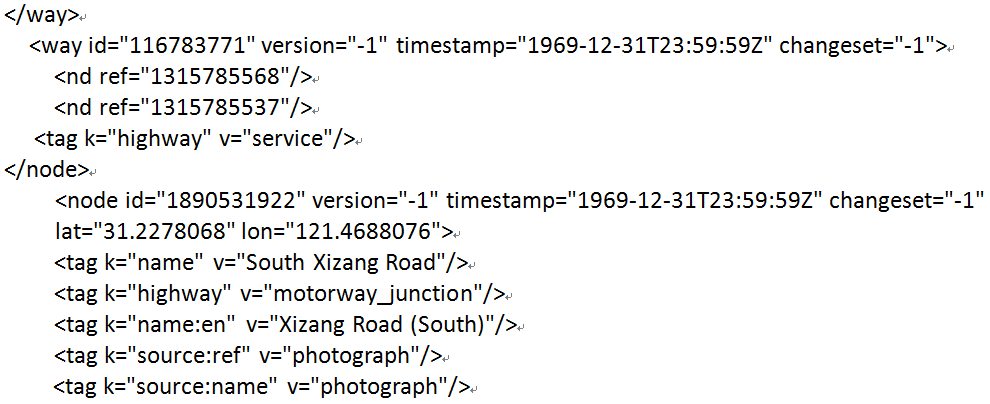
\includegraphics{figures/data/osm_data_format.png}}
	\caption{The OpenStreetMap OSM data format example}
	\label{fig:osmdataformat}
\end{figure}


\subsection{OpenStreetMap}

The open-source OpenStreetMap data dump is available at 
\url{http://planet.osm.org/}. 
%as both a full dataset and a weekly change-set of the planet, 
%showing all the updates that have been made to the planet by contributors. 
%Since in the current stage of the project, all we are interested only in a small area of Eastern China containing Shanghai Municipality, we have used the \url{http://extract.bbbike.org/}, with the same data via the OpenStreetMap API for downloading our raw map data, where the customizable bounding box selection data export is available. The imported bounding box area starts from the south-west corner of approximately longitude 120.027°, latitude 30.551° to the north-east corner of approximately longitude 122.217°, latitude 31.805°.
%\begin{figure}[th]
%	\centering
%	\resizebox{\columnwidth}{!}{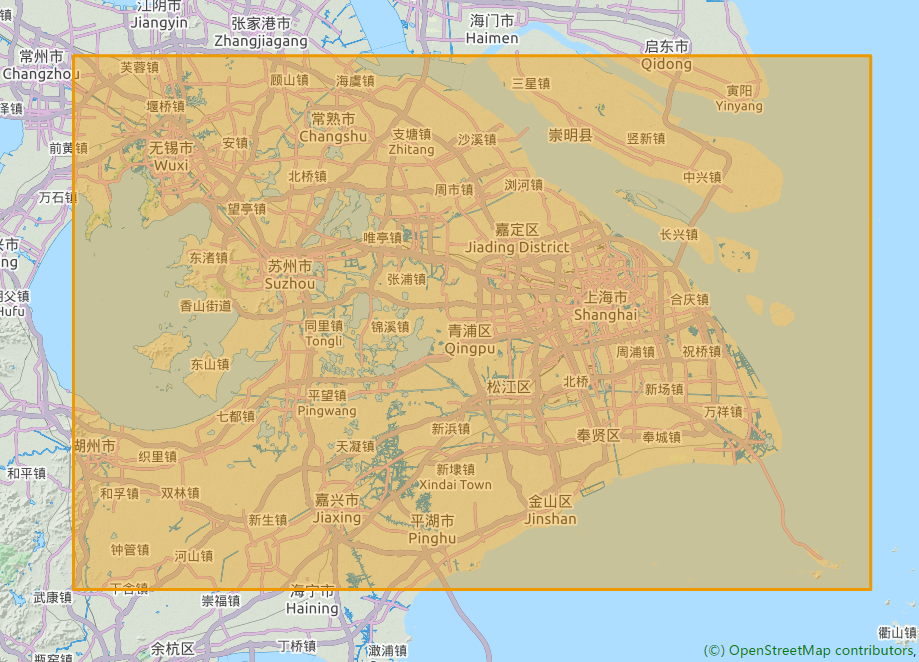
\includegraphics{figures/data/data_extract_bbox.png}}
%	\caption{The bounded area of OSM data dump export}
%	\label{fig:datadumpbbox}
%\end{figure}
%is named as OSM XML format, a format for storing vector map road raw data. First of all, it is XML, XML is a so called meta format to provide even human readable data interexchange formats. Various file formats use this data tree structure to embed their data. The major tools in the OSM universe use an XML format following a XML schema definition that was first used by the API only. Basically it is a list of instances of our data primitives (nodes, ways, and relations). The contents of the file format include the following several parts: 
%
%\begin{itemize}\itemsep0pt
%	\item an XML suffix introducing the UTF-8 character encoding for the file
%	\item an OSM element, containing the version of the API (and thus the features used) and the generator that distilled this file (e.g. an editor tool)
%	\item a block of nodes containing especially the location in the WGS84 reference system
%	\item the tags of each node
%	\item a block of ways
%	\item the references to its nodes for each way
%	\item the tags of each way
%	\item a block of relations
%	\item the references to its members for each relation
%	\item the tags of each relation
%\end{itemize}
The data is in XML format as shown in \figref{fig:osmdataformat}. 
Elements are the basic components of OpenStreetMap's conceptual 
data model of the physical world, also called the data primitives. 
They consist of nodes (defining points in space), 
ways (defining linear features and area boundaries), and 
relations (which are sometimes used to explain how other elements work 
together). All of the above can have one of more associated tags 
(which describe the meaning of a particular element).

A node represents a specific point on the earth's surface defined by 
its latitude and longitude. 
%Each node comprises at least an id number and a pair of coordinates. Nodes can be used to define standalone point features. 
For example, a node could represent a park bench or a water well. 
Nodes are also used to define the shape of a way. 
%When used as points along ways, nodes usually have no tags, though some of them could. For example, highway=traffic\_signals marks traffic signals on a road, and power=tower represents a pylon along an electric power line. 
We mainly use nodes individually and separately to represent 
point features, such as POIs (points of interests). 
%A node can be included as member of relation. The relation also may indicate the member's role: that is, the node's function in this particular set of related data elements.

A way is an ordered list of between 2 and 2,000 nodes that define 
a polyline. Ways are used to represent linear features 
such as rivers and roads. Ways can also represent the boundaries 
of areas (solid polygons) such as buildings or forests. 
%In this case, the way's first and last node will be the same. 
%This is called a ``closed way". Note that closed ways occasionally represent 
%loops, such as roundabouts on highways, rather than solid areas. 
%The way's tags must be examined to discover which it is. 
What we mainly focus on and utilize are the ways 
with specific tag ``highway'', 
which identifies any kind of road, street or path.
For example, highway=residential defines a local road connecting 
homes within a residential area. 
The highway key is associated with values which indicate the 
importance of the highway within the road network. 
%Areas with holes, or with boundaries of more than 2,000 nodes, 
%cannot be represented by a single way. Instead, 
%the feature will require a more complex multi-polygon relation data structure.

A relation is a multi-purpose data structure that documents 
a relationship between two or more data elements 
(nodes, ways, and/or other relations). 
Examples include: A route relation, which lists the ways that form a 
major (numbered) highway, a cycle route, or a bus route. 
%A turn restriction that says you can't turn from one way into another way. 
%A multi-polygon that describes an area (whose boundary is the 'outer way') 
%with holes (the 'inner ways'). Thus, relations can have different meanings. 
%The relation's meaning is defined by its tags. Typically, 
%the relation will have a 'type' tag. 
%The relation's other tags need to be interpreted in light of the type tag. 
A relation is essentially an ordered list of nodes, ways, 
or other relations. 
These objects are known as the relation's members. 
%Each element can optionally have a role within the relation. 
%For example, a turn restriction would have members with ``from" and 
%``to" roles, describing the particular turn that is forbidden. 
%A single element such as a particular way may appear multiple times in 
%a relation.

%Besides the basic nodes and ways, our information also requires from another important part of the data format, other than just longitude and latitude, and that is the tags of those basic elements. All types of data element (nodes, ways and relations) can have tags. Tags describe the meaning of the particular element to which they are attached. A tag consists of two free format text fields; a 'key' and a 'value'. Each of these are Unicode strings of up to 255 characters. There is no fixed dictionary of tags, but there are many conventions documented on the OpenStreetMap wiki. If there is more than one way to tag a given feature, it's probably best to use the most common approach.

\subsection{Baidu Map}
%The second part of the raw data collection is clearly the traffic situations, both currently and historically, on all the roads in the road network that we have previously downloaded and constructed from OpenStreetMap data. It is main drawback that such open source mapping service like OpenStreetMap does not provide such data, mainly because that the data source of traffic data is often acquired from taxi or drive GPSs as well as the authorities’ traffic monitoring. So we need a third party data provider with most reliable traffic data. As the main study area is Shanghai now, after investigating various real-time traffic information provider, including Google Maps, AutoNavi and Bing Maps, etc., 
While OSM serves as the basis of the map structures, due to the 
cultural and government regulations, it has not become the 
most popular choice of mapping software in China, 
and hence its user-generated features such 
as points of interests are extremely deficient. 
Most importantly, OSM doesn't provide live traffic 
conditions in China, which is key for training a prediction
model. Baidu Map, the biggest map provider in China as of 2016, 
on the contrary, has all the bells and whistles. 
Baidu provides a number of web APIs. We use the following APIs in this
work. One is coordinate conversion API used for converting other 
global coordinate systems (e.g., WGS-84 and GCJ-02) to Baidu lon-lat 
coordinates BD-09. The second related API converts BD-09 coordinates
to Baidu's internal (x, y) point coordinates. These internal coordinates
can be used to locate image pixels on Baidu map.
The third API is bounded POI search. 
This API can return all POIs of a certain category
within an area bound by longitudes and latitudes entered by users.
Baidu map has a two level classification of POI types with 18 level-1
types and 123 level-2 POI types.

%After downloading all the POI data using Baidu Maps API, we processed the 
%data with a script, removing the duplicates and then load all the data 
%into our database, each place as a node mentioned earlier, 
%with tags source=baidu and poitype=* and longitude and latitude. 

\begin{figure}[th]
	\centering
	\resizebox{0.9\columnwidth}{!}{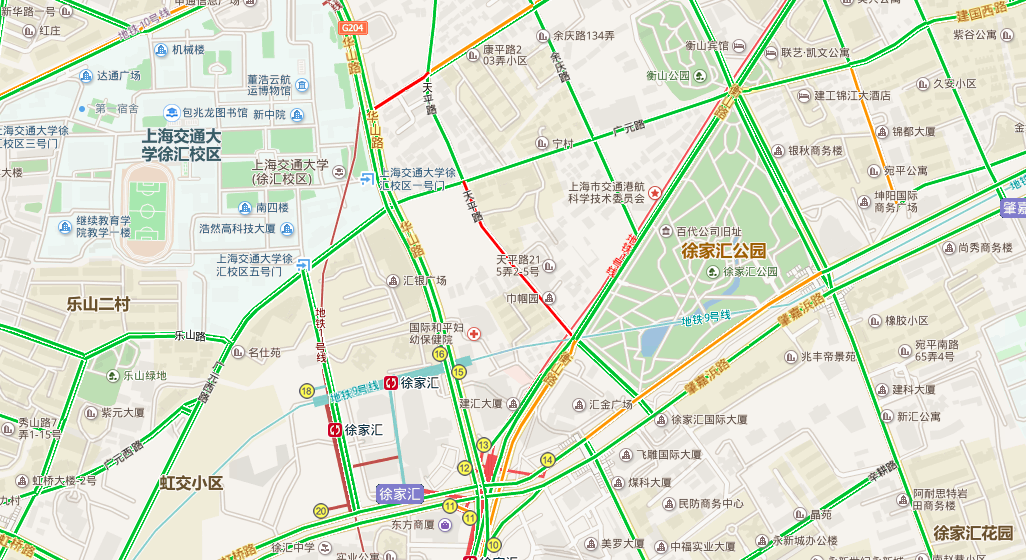
\includegraphics{figures/data/baidutraffic.png}}
	\caption{Part of Shanghai on Baidu Map with live traffic}
	\label{fig:baidutraffic}
\end{figure}

Baidu also provides near real-time traffic condition information, updates
by the minute. For example in \figref{fig:baidutraffic}, green, 
yellow, red and deep red lines represent
clear, slow, congested and extremely congested traffic. 
Programmatically, the traffic information can be obtained by 
two image APIs:
\begin{itemize}\itemsep0pt
	\item Map image API in form of 
		\path{http://online1.map.bdimg.com/onlinelabel/?qt=tile&x=13204&y=3550&z=16}. 
		See \figref{fig:baidutile} for returned image.
	\item Traffic image API in form of 
		\path{http://its.map.baidu.com:8002/traffic/TrafficTileService?level=16&x=13204&y=3550&time=1464020567811}. See \figref{fig:baidutraffictile} for returned image.
\end{itemize}

Each of the APIs returns a $256\times256$ pixels image tile given 
a pair of $(x, y)$ coordinates and a zoom level. 
With the same $x$ and $y$ and zoom level, the two APIs return 
tiles of the same physical size and in the same location, such as shown in
\figref{fig:imageapi}.

\begin{figure}[th]
	\centering
	\begin{subfigure}[t]{0.45\columnwidth}
	\framebox{\resizebox{\columnwidth}{!}{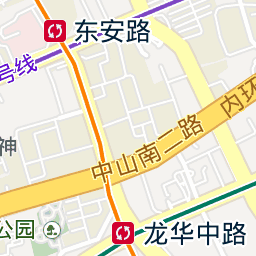
\includegraphics{figures/data/tile.png}}}
	\caption{256*256 px map tile}
	\label{fig:baidutile}
	\end{subfigure}
	\hfill
	\begin{subfigure}[t]{0.45\columnwidth}
	\framebox{\resizebox{\columnwidth}{!}{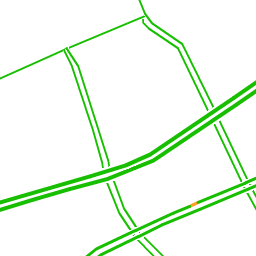
\includegraphics{figures/data/traffictile.png}}}
	\caption{256*256 px traffic tile}
	\label{fig:baidutraffictile}
	\end{subfigure}
    \caption{Image tiles at same location, returned by the image APIs}
    \label{fig:imageapi}
\end{figure}

%
%As you can see, the first API retrieves the tile image of the Baidu Map at given place (defined as tile coordinate x and y) and given zoom z. The second API is the traffic tile image overlay API that provides a PNG image with just polylines with color representing the traffic situation, with given x, y, z, along with a time parameter. We have a crawler that continuously download those data of the whole Shanghai urban area, getting tiles at zoom level 18 and composes all of those small tiles and traffic overlay into a large image. Because all the retrieve data are in raster image format, the next step would be parsing them using some image processing libraries.
